\documentclass[a4paper,12pt]{article}

\usepackage{fontspec}
\newfontfamily{\defaultfont}{CMU Serif}
\newfontfamily{\thaifont}[Scale=MatchLowercase]{TH Sarabun Chula}

\usepackage{polyglossia}
\setdefaultlanguage{thai}
\setotherlanguages{english}

\usepackage[Latin,Thai]{ucharclasses}
\setDefaultTransitions{\defaultfont}{}
\setTransitionTo{Thai}{\thaifont}

\XeTeXlinebreaklocale "th"
\XeTeXlinebreakskip = 0pt plus 0pt

\linespread{1.25}

\usepackage{amsmath,amsthm,amssymb}
\usepackage[ISO]{diffcoeff}
\usepackage{siunitx}
\usepackage[margin=1in]{geometry}
\usepackage{graphicx}
\usepackage{hyperref}
\pagenumbering{gobble}
\begin{document}

\noindent\textbf{ข้อ 2} มวล \(m\) เคลื่อนที่มาบนพื้นราบลื่นด้วยอัตราเร็ว \(u_0\) ยกเว้นพื้นช่วง AB มีความฝืด โดยสัมประสิทธิ์ความเสียดทานจลน์เท่ากับ \(\mu\) เมื่อมวล \(m\) เคลื่อนที่ผ่านพื้นช่วง AB ปรากฏว่ามวล \(m\) ถูกเกี่ยวด้วยสปริงตะขอมีจนาดเท่ากับ \(\dfrac{\mu mg}{\ell}\) และเมื่อสปริงยาวขึ้นเป็น \(2\ell\) ทำให้มวล \(m\) ลอยขึ้นจากพื้นสูงสุดพอดี\\\\
(กำหนดให้ \(u_0=\sqrt{6\mu h\ell}\)) จงหา
\begin{enumerate}
	\item ขนาดของความเร็วมวล \(m\) ขณะเริ่มเกี่ยวกับปลายล่างสปริง
	\item ความสูงของมวล \(m\) ที่แกว่งได้ขึ้นไปสูงสุดจากพื้น
\end{enumerate}
\begin{figure}[h]
	\centering
	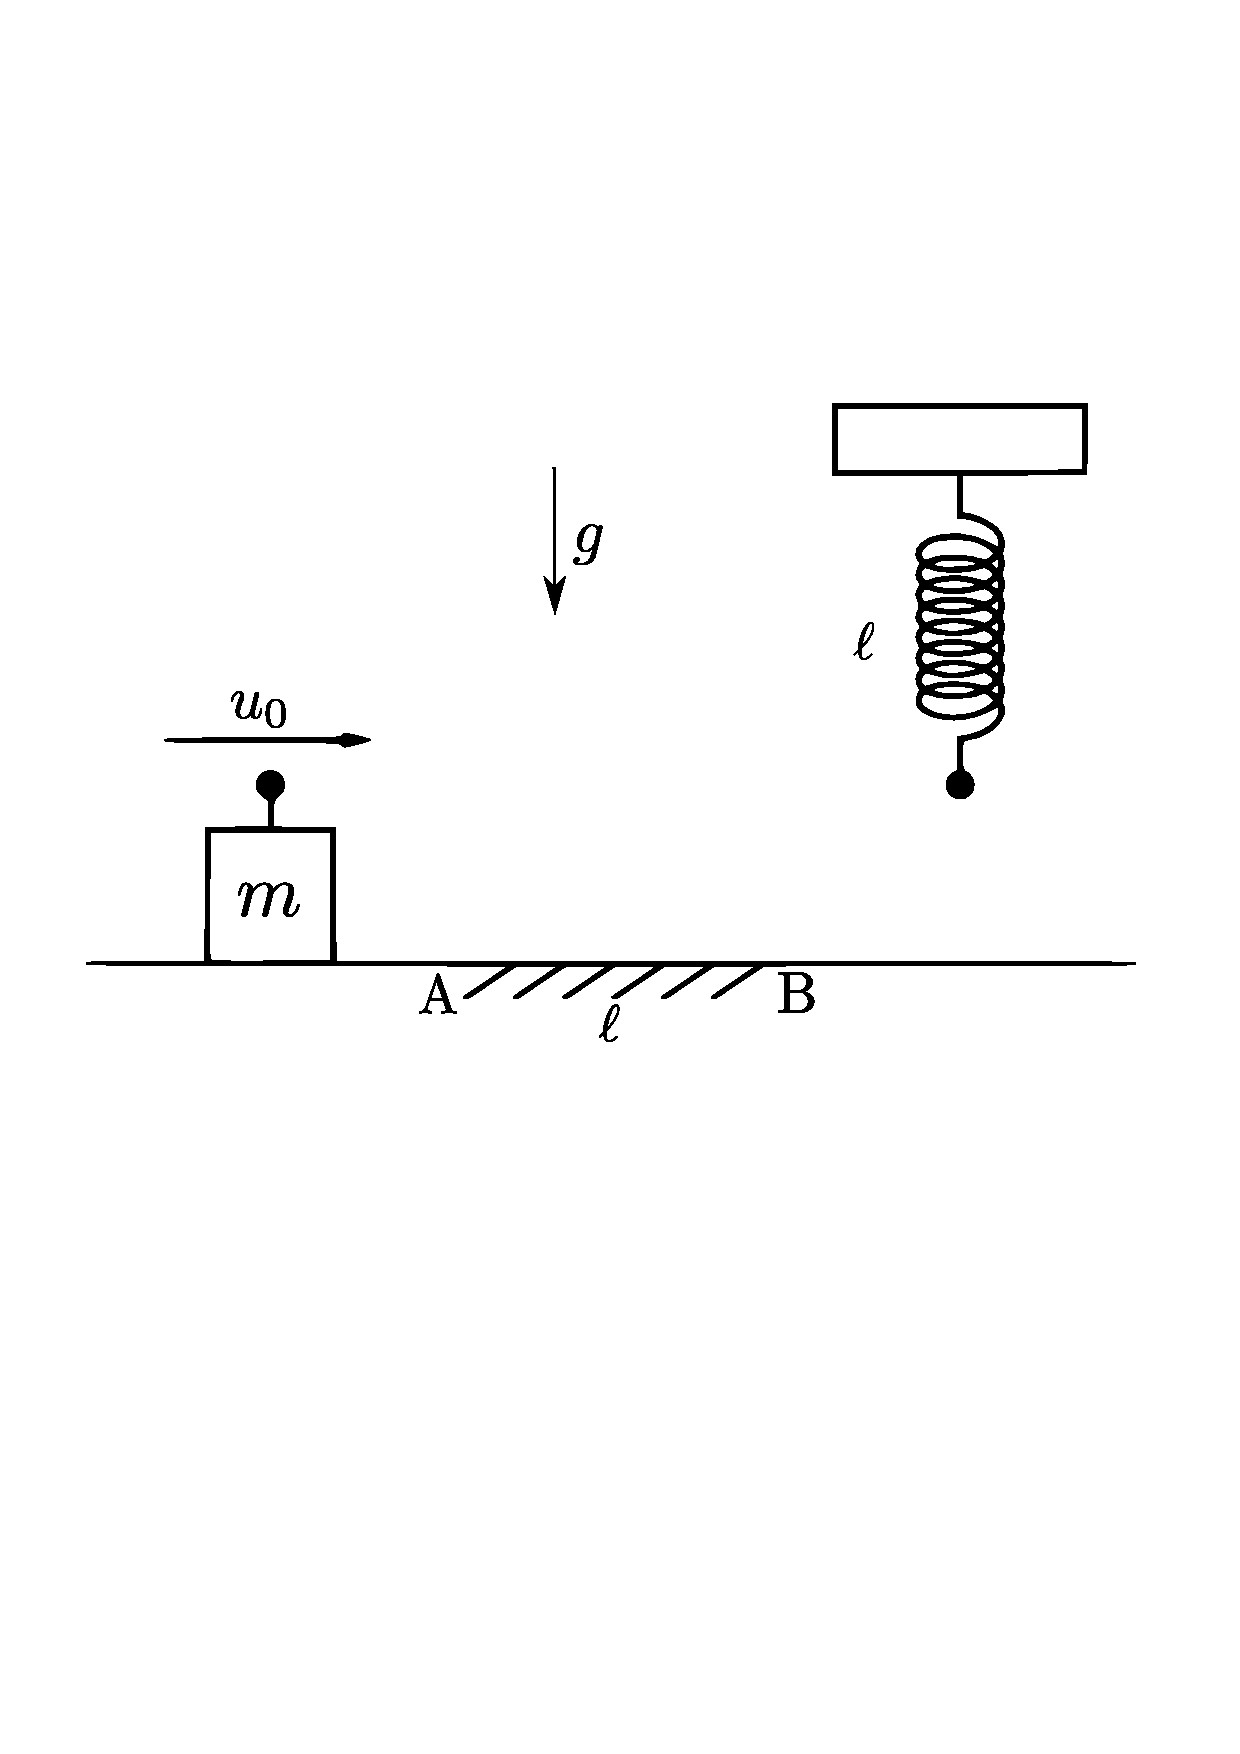
\includegraphics[width=0.5\linewidth]{problem1}
\end{figure}

\end{document}